\documentclass{book}
\usepackage{xeCJK}
\usepackage{ctexcap}
\usepackage{bm}
\usepackage{amsmath,amssymb,amsfonts}
\usepackage{float}

\begin{document}
\chapter{电力系统中的特种变压器}

前面各章讨论的都是每相一个一次绕组和一个二次绕组的双绕组变压器,本章将介绍几 种常见的、在结构或用途上不同于普通双绕组电力变压器的特种变压器。

\section{自耦变压器}

\subsection{结构特点}

普通的双绕组变压器,一、二次侧独立分开,一次绕组匝数为${{N}_{1}}$,二次绕组匝数为${{N}_{2}}$,二者之间只有磁的联系,而无电的联系,如图\ref{fig_5-1}(a)所示。而自耦变压器的二次绕组是一次绕组的一部分,如图\ref{fig_5-1}(b)所示。如果其整个绕组的匝数${{N}_{ab}}={{N}_{1}}$,抽头c以下部分的匝数${{N}_{cb}}={{N}_{2}}$,则它可起到与图\ref{fig_5-1}(a)中的双绕组变压器同样的变压作用。

在图\ref{fig_5-1}(b)中,cb称为绕组的公共段,ac称为绕组的串联段。在实际自耦变压器中,ac和cb两段绕组也像双绕组变压器一、二次绕组那样,一里一外地套在铁心柱上,如图\ref{fig_5-1}(c)所示。两段绕组串联在一起作为一次绕组,靠近铁心的一段作二次绕组。显然一、二次绕组之间除有磁的联系外还有电的联系。

\begin{figure}[H]
	\centering
	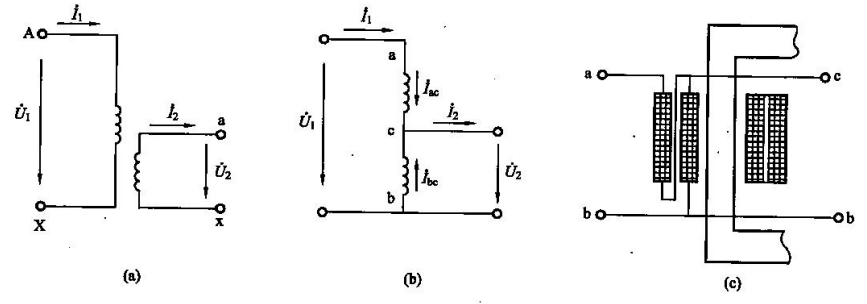
\includegraphics[width=0.80\textwidth]{5-1.png}
	\caption{双绕组变压器与自耦变压器
		(a)无电联系的双绕组变压器;(b)有电联系的双绕组变压器;(c)自耦变压器}
	\label{fig_5-1}
\end{figure}

\subsection{电压、电流关系}


\subsubsection{电压关系}

以降压变压器为例,当把一次绕组接于交流电源时,在铁心中将产生最大值为${{\Phi }_{m}}$的正弦交变磁通,它在一次绕组中产生的感应电动势为
\begin{equation}
{{E}_{1}}={{E}_{ab}}=4.44f{{N}_{ab}}{{\Phi }_{m}}
\label{5-1}
\end{equation}

而在二次绕组(即公共段)中的感应电动势为
\begin{equation}
{{E}_{2}}={{E}_{cb}}=4.44f{{N}_{cb}}{{\Phi }_{m}}
\label{5-2}
\end{equation}

\begin{equation}
\frac{{{E}_{1}}}{{{E}_{2}}}=\frac{{{N}_{ab}}}{{{N}_{cb}}}={{k}_{A}}
\label{5-3}
\end{equation}
式中  ${{k}_{A}}$¬——自耦变压器的变比。

像分析双绕组变压器时一样,如忽略一、二次侧中较小漏阻抗压降,则有${{U}_{1}}\approx {{E}_{1}}{{U}_{2}}\approx {{E}_{2}}$。可见,自耦变压器一、二次侧的电压比也近似地与匝数成正比,即
\begin{equation}
\frac{{{U}_{1}}}{{{U}_{2}}}\approx \frac{{{E}_{1}}}{{{E}_{2}}}\text{=}\frac{{{N}_{ab}}}{{{N}_{cb}}}={{k}_{A}}
\label{5-4}
\end{equation}

串联段上的电压为
\begin{equation}
{{U}_{ab}}={{U}_{1}}-{{U}_{2}}=\left( {{k}_{A}}-1 \right){{U}_{2}}
\label{5-5}
\end{equation}

\subsubsection{电流关系}

为简化分析,忽略较小的励磁电流。根据磁动势平衡,串联段电流所产生的磁动势与公共段电流所产生磁动势应相互抵消为零。这就要求${{\dot{I}}_{ac}}$与${{\dot{I}}_{bc}}$ 同相位,且有
\begin{equation}
{{\dot{I}}_{ac}}{{N}_{1}}={{\dot{I}}_{bc}}{{N}_{2}}
\label{5-6}
\end{equation}

式中  ${{\dot{I}}_{ac}}$¬¬——一次侧的输入电流${{I}_{1}}$。

由于${{N}_{ac}}={{N}_{ab}}-{{N}_{cb}}$,所以公共段中流人的电流为
\begin{equation}
{{I}_{bc}}=\frac{{{N}_{ab}}-{{N}_{cb}}}{{{N}_{cb}}}{{I}_{1}}=\left( {{k}_{A}}-1 \right){{I}_{1}}
\label{5-7}
\end{equation}

而二次侧输出的电流为
\begin{equation}
{{I}_{2}}={{I}_{ab}}+{{I}_{bc}}={{I}_{1}}+\left( {{k}_{A}}-1 \right){{I}_{1}}={{k}_{A}}{{I}_{1}}
\label{5-8}
\end{equation}

可见,在励磁电流可以忽略的条件下,自耦变压器一、二次侧电流也与匝数成反比,即
\begin{equation}
\frac{{{I}_{1}}}{{{I}_{2}}}\approx \frac{1}{{{k}_{A}}}=\frac{{{N}_{cb}}}{{{N}_{ab}}}
\label{5-9}
\end{equation}

比较式(\ref{5-7})和式(\ref{5-8})可知,公共段绕组中流过的电流${{I}_{bc}}$小于二次侧输出电流${{I}_{2}}$,等于${{I}_{2}}-{{I}_{1}}$。

\subsection{感应功率和传导功率}

在普通双绕组变压器中,能量的传递全部经过磁路由电磁感应来完成,即二次侧得到的 电功率全部为感应功率。而在自耦变压器中;一部分能量是通过电磁感应传递,具体表现为 ac和bc两段绕组中的磁动势平衡;另一部分能量则直接由电源传递到负载。由此说明,负 载同时得到两部分电功率,前者为感应功率,后者为传导功率。

变压器二次侧输出的视在功率为
\begin{equation}
{{S}_{2}}={{U}_{2}}{{I}_{2}}={{U}_{2}}{{I}_{ac}}+{{U}_{2}}{{I}_{bc}}
\label{5-10}
\end{equation}

其中${{I}_{ac}}={{I}_{1}}$

式中  ${{I}_{ac}}$——一次侧电流,它流过串联段绕组 ac后,直接流到负载中(见图\ref{fig_5-2}),与${{I}_{ac}}$对应的输出功率${{U}_{2}}{{I}_{ac}}$为传导功率。

\begin{figure}[H]
	\centering
	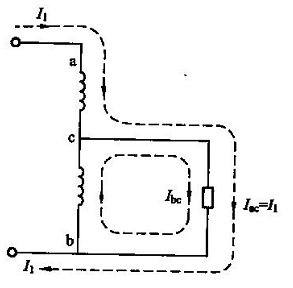
\includegraphics[width=0.80\textwidth]{5-2.png}
	\caption{自耦变压器的电流路径}
	\label{fig_5-2}
\end{figure}

由于${{I}_{ac}}={{I}_{1}}=\frac{1}{{{k}_{A}}}{{I}_{2}}$,所以传导功率与整个输出功率之比为
\begin{equation}
\frac{{{U}_{2}}{{I}_{ac}}}{{{U}_{2}}{{I}_{2}}}=\frac{1}{{{k}_{A}}}
\label{5-11}
\end{equation}

当${{I}_{1}}$通过串联段ac时,在公共段cb中将产生感应电流${{I}_{bc}}$,其大小取决于两段间的磁动势平衡。在忽略励磁电流的条件下,其值为
\begin{equation}
{{I}_{bc}}=\left( {{k}_{A}}-1 \right){{I}_{1}}=\frac{{{k}_{A}}-1}{{{k}_{A}}}\times {{I}_{2}}=\left( 1-\frac{1}{{{k}_{A}}} \right){{I}_{2}}
\label{5-12}
\end{equation}

与${{I}_{bc}}$对应的输出功率${{U}_{2}}{{I}_{bc}}$为感应功率,它与整个输出功率的比值为
\begin{equation}
\frac{{{U}_{2}}{{I}_{bc}}}{{{U}_{2}}{{I}_{2}}}=1-\frac{1}{{{k}_{A}}}
\label{5-13}
\end{equation}

由式(\ref{5-11})和式(\ref{5-13})可知,当自耦变压器的变比${{k}_{A}}$增大时,传导功率变小,而感应功率变大。

\subsection{自耦变压器的短路阻抗}

在应用简化等效电路进行分析计算时,必须先知道变压器的短路阻抗。在双绕组变压器 中短路阻抗${{Z}_{k}}={{Z}_{1}}+{{{Z}'}_{2}}$,而在自耦变压器中将不再有这样的关系。


\begin{figure}  
	\begin{minipage}[H]{0.45\linewidth}  
		\centering  
		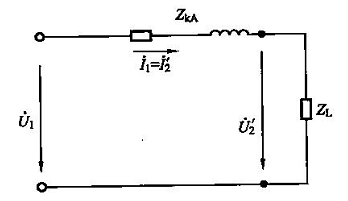
\includegraphics[width=2.2in]{5-3.png}  
		\caption{自耦变压器的简化等效电路}  
		\label{fig:5-3}  
	\end{minipage}
	\begin{minipage}[H]{0.45\linewidth}  
		\centering  
		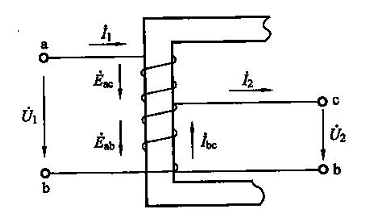
\includegraphics[width=2.2in]{5-4.png}  
		\caption{自耦变压器各主要物理量间的关系}  
		\label{fig:5-4}  
	\end{minipage}  
\end{figure}

图\ref{fig:5-3}所示为自耦变压器的简化等效电路,而电路中短路阻抗上的电压降为
\begin{equation}
{{\dot{I}}_{1}}{{Z}_{kA}}={{\dot{U}}_{1}}-{{{\dot{U}}'}_{2}}
\label{5-14}
\end{equation}

为了确定${{Z}_{kA}}$ 的大小,应先列出${{\dot{U}}_{1}}$ 和${{\dot{U}}_{2}}$ 的表达式。按图\ref{fig:5-4}中所标注的正方向,可列出自耦变压器一、二次侧的电压平衡方程式和各电流之间的关系,它们分别为
\begin{equation}
{{\dot{U}}_{1}}\text{=}\left( \text{-}{{{\dot{E}}}_{ab}} \right)+{{\dot{I}}_{1}}{{Z}_{ab}}+\left( -{{{\dot{I}}}_{bc}} \right){{Z}_{cb}}
\label{5-15}
\end{equation}

\begin{equation}
\left( -{{{\dot{E}}}_{cb}} \right)={{\dot{U}}_{2}}+{{\dot{I}}_{bc}}{{Z}_{cb}}
\label{5-16}
\end{equation}
\begin{equation}
{{\dot{I}}_{1}}+{{\dot{I}}_{bc}}={{\dot{I}}_{2}}
\label{5-17}
\end{equation}

将式(\ref{5-16})乘以${{k}_{A}}=\frac{{{N}_{ab}}}{{{N}_{cb}}}$,并考虑到感应电动势与匝数的正比关系,可得
\begin{equation}
\left( -{{{\dot{E}}}_{ab}} \right)={{\dot{{U}'}}_{2}}+{{k}_{A}}{{\dot{I}}_{bc}}{{Z}_{cb}}
\label{5-18}
\end{equation}

将式(\ref{5-18})代入式(\ref{5-15})得
\begin{equation}
{{\dot{U}}_{1}}={{\dot{{U}'}}_{2}}+\left( {{k}_{A}}-1 \right){{\dot{I}}_{bc}}{{Z}_{cb}}+{{\dot{I}}_{1}}{{Z}_{ac}}
\label{5-19}
\end{equation}

在忽略励磁电流的条件下,根据式(\ref{5-7})可知${{\dot{I}}_{bc}}=\left( {{k}_{A}}-1 \right){{\dot{I}}_{1}}$,于是式(\ref{5-19})可改写为
\begin{equation}
{{\dot{U}}_{1}}={{\dot{{U}'}}_{2}}+{{\dot{I}}_{1}}\left[ {{Z}_{ac}}+{{\left( {{k}_{A}}-1 \right)}^{2}}{{Z}_{cb}} \right]
\label{5-20}
\end{equation}

将式(\ref{5-20})与式(\ref{5-14})对照可以看出自耦变压器短路阻抗的大小为
\begin{equation}
{{Z}_{kA}}={{Z}_{ac}}+{{\left( {{k}_{A}}-1 \right)}^{2}}{{Z}_{cb}}
\label{5-21}
\end{equation}

设图(\ref{fig_5-1}(a))中的双绕组变压器与图\ref{fig_5-1}(b)中的自耦变压器容量相等,一、二次侧额定电压也分别相等,现在来比较它们的短路阻抗值。双绕组变压器的短路阻抗为
\begin{equation}
{{Z}_{k}}={{Z}_{1}}+{{{Z}'}_{2}}={{Z}_{1}}+{{k}^{2}}{{Z}_{2}}
\label{5-22}
\end{equation}

根据假设可知${{k}_{A}}=k$,由${{N}_{cb}}={{N}_{2}}$ 可知${{Z}_{cb}}={{Z}_{2}}$,所以${{\left( {{k}_{A}}-1 \right)}^{2}}{{Z}_{cb}}<{{k}^{2}}{{Z}_{2}}$ ;由于${{N}_{ac}}<{{N}_{1}}$,所以${{Z}_{ac}}<{{Z}_{1}}$。既然式(\ref{5-21})右端两项都分别小于式(\ref{5-22})右端的两项,可见自耦变压器的短路阻抗${{Z}_{kA}}$小于同容量的双绕组变压器的短路阻抗${{Z}_{k}}$。二者相差的多少取决于变比的大小,变比越小,它们相差得越多。

\begin{figure}[H]
	\centering
	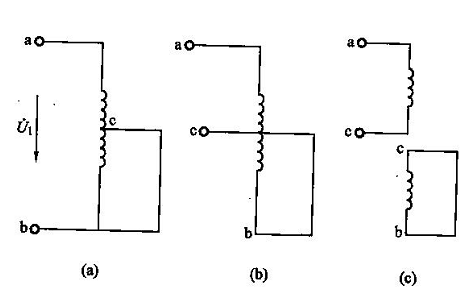
\includegraphics[width=0.80\textwidth]{5-5.png}
	\caption{自耦变压器的短路试验
		(a)接线图;(b)等效电路一;(c)等效电路二}
	\label{fig_5-5}
\end{figure}
自耦变压器的短路阻抗也可以通过短路试验来测定,图\ref{fig_5-5}(a)为其接线图,图\ref{fig_5-5}(b)、(c)为其等效电路图。通过电路的等效变换可见,自耦变压器短路时,相当于以串联段ac为一次侧,公共段cb为二次侧的双绕组变压器。短路阻抗应等于ac段的电抗加上cb段阻抗归算到ac段后的值,即${{Z}_{kA}}={{Z}_{ac}}+{{\left( \frac{{{N}_{ac}}}{{{N}_{cb}}} \right)}^{2}}{{Z}_{cb}}$ ,由于$\frac{{{N}_{ac}}}{{{N}_{cb}}}=\frac{{{N}_{ab}}-{{N}_{cb}}}{{{N}_{cb}}}={{k}_{A}}-1$可见,由短路试验测得的${{Z}_{kA}}$值与式(\ref{5-21})完全相同。

\subsection{自耦变压器的优、缺点和应用范围}

1.主要优点

仍以图\ref{fig_5-1}(a)、(b)中的两台变压器作比较,自耦变压器的主要优点如:

(1)节省材料。自耦变压器串联段 ac 中的电流与双绕组变压器一次侧AX中的电流相 同,所以它们所用导线的截面积相等,两者的用铜(或铝)量正比于导线的长度,也就是正 比于绕组的匝数,即
\begin{equation}
\frac{{{G}_{ac}}}{{{G}_{AX}}}=\frac{{{N}_{ac}}}{{{N}_{1}}}=\frac{{{N}_{ab}}-{{N}_{cb}}}{{{N}_{ab}}}=1-\frac{1}{{{k}_{A}}}
\label{5-23}
\end{equation}

自耦变压器公共段cb与双绕组变压器二次侧 ax 的匝数相等,二者的用铜(或铝)量与它们的导线截面积成正比。而导线的截面积是根据它所通过电流的大小而定,所以
\begin{equation}
\frac{{{G}_{cb}}}{{{G}_{ax}}}=\frac{{{I}_{bc}}}{{{I}_{2}}}=\frac{\left( {{k}_{A}}-1 \right){{I}_{1}}}{k{{I}_{1}}}=1-\frac{1}{{{k}_{A}}}
\label{5-24}
\end{equation}


由式(\ref{5-23})和式(\ref{5-24})可知,自耦变压器绕组所用材料比同容量的双绕组变压器节省$\frac{1}{{{k}_{A}}}$。而$\frac{1}{{{k}_{A}}}$恰是传导功率在整个功率中所占的比率,这说明绕组的材料用量只取决于感应功率的大小。

(2)效率高。比较自耦变压器串联段ac与双绕组变压器一次侧绕组的 AX 中的铜损耗,它们的比值为
\begin{equation}
\frac{{{p}_{Cuac}}}{{{p}_{CuAX}}}=\frac{I_{1}^{2}{{r}_{ac}}}{I_{1}^{2}{{r}_{1}}}=\frac{{{N}_{ac}}}{{{N}_{1}}}=\frac{{{N}_{ab}}-{{N}_{cb}}}{{{N}_{ab}}}=1-\frac{1}{{{k}_{A}}}
\label{5-25}
\end{equation}

再比较自耦变压器公共段cb与双绕组变压器二次侧ax中的铜损耗。二者的电阻与导线截面成反比,也就是与流过其中的电流成反比,所以有
\begin{equation}
\frac{{{p}_{Cucb}}}{{{p}_{Cuax}}}=\frac{I_{bc}^{2}{{r}_{cb}}}{I_{2}^{2}{{r}_{2}}}=\frac{I_{bc}^{2}{{I}_{2}}}{I_{2}^{2}{{I}_{bc}}}=\frac{{{I}_{bc}}}{{{I}_{2}}}=\frac{{{I}_{2}}-{{I}_{1}}}{{{I}_{2}}}=1-\frac{1}{{{k}_{A}}}
\label{5-26}
\end{equation}

式(\ref{5-23})和式(\ref{5-26})表明,自耦变压器铜损耗的减小与其材料的节省具有相同的比率。${{k}_{A}}$越小,铜损耗越小,效率越高。

(3)电压变化率小。由于自耦变压器的短路阻抗${{Z}_{kA}}$比同容量的双绕组变压器小,所以在运行时电压变化率较小。

2. 主要缺点

(1)一、二次侧有电的联系。在故障情况下,二次绕组与其连接的各种设备都有可能经受到全部高压,这就提高了对它们的绝缘要求。变比${{k}_{A}}$越大,这个缺点就越突出。另外,当一方遭受过电压时立即波及另一方,故其过电压保护比双绕组变压器复杂。

(2)短路电流大。由于自耦变压器的短路阻抗较小,所以在发生短路时会产生比双绕组变压器更大的电流。

3. 适用场合

根据上面的分析可以看出,自耦变压器只有在变化较小时其优点才显著,而在变比较大时其第一个缺点变得更为突出。因此自耦变压器主要用于变比较小的场合。

在实验室中,大量使用可调的自耦变压器作为可变电压的电源。为限制交流电动机的起 动电流,也广泛采用三相自耦变压器来降低起动时的电压。

\begin{figure}[H]
	\centering
	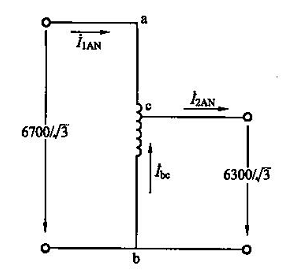
\includegraphics[width=0.80\textwidth]{5-6.png}
	\caption{自耦变压器的一相电路}
	\label{fig_5-6}
\end{figure}

图\ref{fig_5-6}所示为自耦变压器一相电路,其变化为
${{k}_{A}}=\frac{6700/\sqrt{3}}{6300/\sqrt{3}}=1.062$

因为串联段 ac 就是原来的低压绕组,所以自耦变压器高压端的额定电流就等于原双绕组变压器低压端的额定电流,即${{I}_{1AN}}={{I}_{2N}}=\frac{{{S}_{N}}}{\sqrt{3}{{U}_{2N}}}=\frac{320\times {{10}^{3}}}{\sqrt{3}\times 400}=462\left( A \right)$ 

${{S}_{AN}}=\sqrt{3}\times 6700\times 462=5360000\left( V\cdot A \right)=5360\left( kV\cdot A \right)$ 

(3)因为自耦变压器的短路阻抗${{Z}_{kA}}={{Z}_{ac}}+{{\left( \frac{{{W}_{ac}}}{{{W}_{cb}}} \right)}^{2}}{{Z}_{bc}}$,可见它等于以串联段 ac 为一次侧,公共段 cb 为二次侧的双绕组变压器的短路阻抗${{Z}_{k}}$,因此有

${{r}_{kA}}={{r}_{k}}=r_{k}^{*}\frac{{{U}_{2N}}/\sqrt{3}}{{{I}_{2N}}}$

${{x}_{kA}}={{x}_{k}}=x_{k}^{*}\frac{{{U}_{2N}}/\sqrt{3}}{{{I}_{2N}}}$

其标幺值为

$r_{kA}^{*}=\frac{{{r}_{kA}}{{I}_{1AN}}}{{{U}_{1AN}}/\sqrt{3}}=r_{k}^{*}\frac{{{U}_{2N}}}{{{U}_{1AN}}}=0.0178\times \frac{400}{6700}=0.00106$

$x_{kA}^{*}={{x}_{kA}}\frac{{{I}_{1AN}}}{{{U}_{1AN}}/\sqrt{3}}=x_{k}^{*}\frac{{{U}_{2N}}}{{{U}_{1AN}}}=0.052\times \frac{400}{6700}=0.0031$

电压变化率为

\begin{align}
& \Delta U=r_{kA}^{*}\cos {{\varphi }_{2}} \\ 
& =0.00106\times 0.8+0.0031\times 0.6=0.00085+0.00186=0.271\%
\label{}
\end{align}

由于自耦变压器二次侧额定电流为
${{I}_{2AN}}=\frac{{{S}_{AN}}}{\sqrt{3}{{U}_{2AN}}}=\frac{\sqrt{3}{{U}_{1AN}}{{I}_{1AN}}}{\sqrt{3}{{U}_{2AN}}}=\frac{\left( {{U}_{2N}}+{{U}_{1N}} \right){{I}_{2N}}}{{{U}_{1N}}}={{I}_{2N}}+\frac{{{U}_{2N}}{{I}_{2N}}}{{{U}_{1N}}}={{I}_{2N}}+{{I}_{1N}}$

所以在额定运行时公共段cb中的电流等于改变前高压绕组的额定电流

${{I}_{bcN}}={{I}_{2AN}}={{I}_{1AN}}={{I}_{2N}}+{{I}_{1N}}-{{I}_{2N}}={{I}_{1N}}$
既然在改装为自耦变压器前、后两段绕组中的额定电流不变,那么改装后的铜损耗也应不变。另外,由于改装后的额定电压与匝数成正比变化,铁心中主磁通最大值${{\Phi }_{m}}\approx \frac{{{U}_{1}}}{4.44f{{N}_{1}}}$ 将不变,因而铁损耗也不会改变。自耦变压器的效率为

${{\eta }_{A}}=\frac{{{S}_{AN}}\cos {{\varphi }_{2}}}{{{S}_{AN}}\cos {{\varphi }_{2}}+{{p}_{0}}+{{p}_{kN}}}=\frac{5360\times 0.8}{5360\times 0.8+1.45+5.7}=99.83\%$

\section{三绕组变压器}
\subsection{概述}
\subsubsection{用途}

在电力系统中,常常需要通过变压器把三种电压级不同的电网联系起来、有时发电厂产 生的电能需要同时向两个电压不同的高压电网输出。为此,在上述情况下可采用一台三绕组的变压器来代替两台变比不同的双绕组变压器。一台三绕组变压器与它所代替的两台双绕组变压器相比,其主要特点是材料用量少、总体积变小、成本降低。特别是在将两个二次侧输出的高峰错开时,一次侧的容量就可比两二次侧的容量之和小很多。另外,这样替换后还可使发电厂和变电所的设备简化,维护管理方便。因此,三绕组变压器在电力系统中得到广泛的使用。

\subsubsection{结构特点}

三绕组变压器的磁路系统与双绕组变压器相同,只是在每个铁心柱上同心地安放着三个绕组,即高压绕组1、中压绕组2和低压绕组3、如图\ref{fig:5-7}所示。对于升压变压器,为了使 一次侧3和两个二次倒都有较好的耦合关系,因而把低压绕组3由里层移至中间,见图\ref{fig:5-7}(a)所示。对于降压变压器,从绝缘的角度考虑,高压绕组1总是放在最外层,而低压绕组3应放在最里面,如图\ref{fig:5-7}(b)所示。
\begin{figure}  
	\begin{minipage}[H]{0.45\linewidth}  
		\centering  
		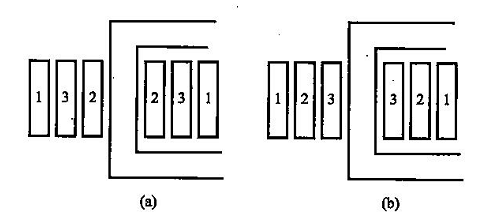
\includegraphics[width=2.2in]{5-7.png}  
		\caption{三绕组变压器的绕组布置图
			(a)升压变压器(b)降压变压器}  
		\label{fig:5-7}  
	\end{minipage}
	\begin{minipage}[H]{0.45\linewidth}  
		\centering  
		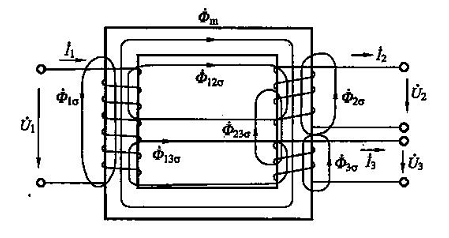
\includegraphics[width=2.2in]{5-8.png}  
		\caption{三绕组变压器电磁关系示意图}  
		\label{fig:5-8}  
	\end{minipage}  
\end{figure}
根据国家标准规定,三相三绕组变压器的标准连接组为YNyn0d11和YNyn0y0两种。

\subsubsection{绕组容量的配合关系 }

根据电力系统运行的实际需要,在三绕组变压器中三个绕组的容量可以设计成相等,也可以不相等。变压器的额定容量是指三相绕组中容量最大的一个绕组的容量。按国际标准规定,三相绕组的容量配合关系有下列三种:

高压绕组	100\%   	100\%	100\%

中压绕组	100\%	    50\%	100\%

低压绕组	50\%	    100\%	100\%

在实际运行中,有时需向某一个二次侧多输出些功率,而向另一个二次侧少输出些功率。无论两个二次侧输出如何变动,只要两个二次侧电流都不超过各自的额定值,两个二次侧电流归算至一次侧的相量和不超过一次侧额定电流,都属于变压器的正常运行。

\subsection{基本电磁关系}

以降压变压器为例,图\ref{fig:5-8}所示为其电磁关系示意图。

\subsubsection{磁动势平衡关系}

一次侧的磁动势${{\dot{F}}_{1}}={{\dot{I}}_{1}}{{N}_{1}}$在抵消二次侧磁动势${{\dot{F}}_{2}}={{\dot{I}}_{2}}{{N}_{2}}$ 和${{\dot{F}}_{3}}={{\dot{I}}_{3}}{{N}_{3}}$之后,保持一定的励磁磁动势${{\dot{F}}_{m}}={{\dot{I}}_{m}}{{N}_{1}}$,以保证主磁通最大值${{\Phi }_{m}}$基本不变。磁动势平衡方程式为
\begin{equation}
{{\dot{F}}_{1}}-{{\dot{F}}_{2}}-{{\dot{F}}_{3}}={{\dot{F}}_{m}}
\label{5-27}
\end{equation}

除以一次侧匝数${{N}_{1}}$,得
\begin{equation}
{{\dot{I}}_{1}}-{{{\dot{I}}'}_{2}}-{{{\dot{I}}'}_{3}}={{\dot{I}}_{m}}
\label{5-28}
\end{equation}

式中  ${{\dot{I}}_{2}}$——${{\dot{I}}_{2}}$归算到一次侧的值,${{{\dot{I}}'}_{2}}=\frac{{{N}_{2}}}{{{N}_{1}}}{{\dot{I}}_{2}}={{k}_{12}}{{\dot{I}}_{2}}$;

${{\dot{I}}_{3}}$——\[{{\dot{I}}_{3}}\]归算到一次侧的值,\[{{{\dot{I}}'}_{3}}=\frac{{{N}_{3}}}{{{N}_{1}}}{{\dot{I}}_{3}}={{k}_{13}}{{\dot{I}}_{3}}\]。

当忽略励磁电流${{I}_{m}}$时,则有
\begin{equation}
{{\dot{I}}_{1}}-{{{\dot{I}}'}_{2}}-{{{\dot{I}}'}_{3}}=0
\label{5-29}
\end{equation}

\subsubsection{电压平衡关系}
由图\ref{fig:5-8}可见,在三绕组变压器中,除主磁通${{\dot{\Phi }}_{m}}$和各绕组的自漏磁${{\dot{\Phi }}_{1\sigma }}{{\dot{\Phi }}_{2\sigma }}{{\dot{\Phi }}_{3\sigma }}$外,还有与两个绕组连接的互漏磁${{\dot{\Phi }}_{12\sigma }}{{\dot{\Phi }}_{13\sigma }}{{\dot{\Phi }}_{23\sigma }}$。互漏磁通由两个绕组中的电流共同产生,它与两个绕组连接,并在这两个绕组中都产生感应电动势。因此对于三绕组变压器,如果像对双绕组变压器那样列电压方程,将由于互漏磁电动势的存在,使分析变得十分困难。这就必须采用每一绕组的自感系数与各绕组间的互感系数作为基本参数,来建立各绕组的电压平衡方程式。另${{L}_{1}}{{L}_{2}}{{L}_{3}}$为各绕组的自感系数;${{M}_{12}}\text{=}{{M}_{21}}$为1与2绕组间的互感系数;${{M}_{13}}\text{=}{{M}_{31}}$为1与3绕组间的互感系数;${{M}_{23}}\text{=}{{M}_{32}}$为2与3绕组间的互感系数。

按图\ref{fig:5-8}所示的电压。电流正方向,可列出
\begin{align}
& {{{\dot{U}}}_{1}}\text{=}{{r}_{1}}{{{\dot{I}}}_{1}}+j\omega {{L}_{1}}{{{\dot{I}}}_{1}}-j\omega {{M}_{12}}{{{\dot{I}}}_{2}}-j\omega {{M}_{13}}{{{\dot{I}}}_{3}} \\ 
& -{{{\dot{U}}}_{2}}\text{=}{{r}_{2}}{{{\dot{I}}}_{2}}+j\omega {{L}_{2}}{{{\dot{I}}}_{2}}-j\omega {{M}_{12}}{{{\dot{I}}}_{1}}+j\omega {{M}_{23}}{{{\dot{I}}}_{3}} \\ 
& -{{{\dot{U}}}_{3}}\text{=}{{r}_{3}}{{{\dot{I}}}_{3}}+j\omega {{L}_{3}}{{{\dot{I}}}_{2}}-j\omega {{M}_{13}}{{{\dot{I}}}_{1}}+j\omega {{M}_{23}}{{{\dot{I}}}_{2}} 
\label{5-30}
\end{align}
式中,1与2之间及1与3之间的互感抗压降取负号,这是因为${{\dot{I}}_{2}}{{\dot{I}}_{3}}$ 流入${{\dot{I}}_{1}}$的流入端不是同极性端。

\subsection{归算及等效电路}
\subsubsection{归算}
为了将绕组2与3中的所有电量和参数都归算到一次侧,需使用三个变化,即
\begin{equation}
{{k}_{12}}=\frac{{{N}_{1}}}{{{N}_{2}}}{{k}_{13}}=\frac{{{N}_{1}}}{{{N}_{3}}}{{k}_{23}}=\frac{{{N}_{2}}}{{{N}_{3}}}
\label{5-31}
\end{equation}

(1)电量与电阻的归算。其归算式分别为
\begin{align}
& {{{{U}'}}_{2}}\text{=}{{k}_{12}}{{U}_{2}}{{{{U}'}}_{3}}\text{=}{{k}_{13}}{{U}_{3}} \\ 
& {{{{I}'}}_{2}}\text{=}\frac{1}{{{k}_{12}}}{{I}_{2}}{{{{I}'}}_{3}}\text{=}\frac{1}{{{k}_{13}}}{{I}_{3}} \\ 
& {{{{r}'}}_{2}}\text{=}k_{12}^{2}{{r}_{2}}{{{{r}'}}_{3}}\text{=}k_{13}^{2}{{r}_{3}} 
\label{5-32}
\end{align}

(2)自感系数的归算。因为${{L}_{2}}$ 正比于$N_{2}^{2}$,${{L}_{3}}$ 正比于
$N_{3}^{2}$,而归算后的${{{L}'}_{2}}$ 和${{{L}'}_{3}}$都正比于$N_{1}^{2}$,所以有
\begin{equation}
{{{L}'}_{2}}=k_{12}^{2}{{L}_{2}},{{{L}'}_{3}}=k_{13}^{2}{{L}_{3}}
\label{5-33}
\end{equation}

(3)互感系数的归算。因为${{M}_{12}}$ 正比于${{N}_{1}}{{N}_{2}}$,${{M}_{13}}$ 正比于${{N}_{1}}{{N}_{3}}$,${{M}_{23}}$正比于${{N}_{2}}{{N}_{3}}$,而归算后的${{{M}'}_{12}}$、${{{M}'}_{13}}$、${{{M}'}_{23}}$都应正比于$N_{1}^{2}$,所以有
\begin{align}
& {{{{M}'}}_{12}}=\frac{N_{1}^{2}}{{{N}_{1}}{{N}_{2}}}{{M}_{12}}={{k}_{12}}{{M}_{12}} \\ 
& {{{{M}'}}_{13}}=\frac{N_{1}^{2}}{{{N}_{1}}{{N}_{3}}}{{M}_{13}}={{k}_{13}}{{M}_{13}} \\ 
& {{{{M}'}}_{23}}=\frac{N_{1}^{2}}{{{N}_{2}}{{N}_{3}}}{{M}_{23}}={{k}_{12}}{{k}_{13}}{{M}_{23}} 
\label{5-34}
\end{align}

(4)归算后的电压方程式。将式(2-30)中的第二式乘以${{k}_{12}}$,第三式乘以${{k}_{13}}$,可得
\begin{align}
& {{{\dot{U}}}_{1}}={{r}_{1}}{{{\dot{I}}}_{1}}+j\omega {{L}_{1}}{{{\dot{I}}}_{1}}-j\omega {{{{M}'}}_{12}}{{{{\dot{I}}'}}_{2}}-j\omega {{{{M}'}}_{13}}{{{{\dot{I}}'}}_{3}} \\ 
& -{{{{\dot{U}}'}}_{2}}={{{{r}'}}_{2}}{{{{\dot{I}}'}}_{2}}+j\omega {{{{L}'}}_{2}}{{{{\dot{I}}'}}_{2}}-j\omega {{{{M}'}}_{12}}{{{\dot{I}}}_{1}}+j\omega {{{{M}'}}_{23}}{{{{\dot{I}}'}}_{3}} \\ 
& -{{{{\dot{U}}'}}_{3}}={{{{r}'}}_{3}}{{{{\dot{I}}'}}_{3}}+j\omega {{{{L}'}}_{3}}{{{{\dot{I}}'}}_{3}}-j\omega {{{{M}'}}_{13}}{{{\dot{I}}}_{1}}+j\omega {{{{M}'}}_{23}}{{{{\dot{I}}'}}_{2}} 
\label{5-35}
\end{align}	

\subsubsection{等效电路}
由式(\ref{5-35})可得绕组1到绕组2的电压降$\Delta {{\dot{U}}_{12}}={{\dot{U}}_{1}}-{{{\dot{U}}'}_{2}}$和绕组1到绕组3的电压降$\Delta {{\dot{U}}_{13}}={{\dot{U}}_{1}}-{{{\dot{U}}'}_{3}}$。考虑到${{\dot{I}}_{1}}-{{{\dot{I}}'}_{2}}-{{{\dot{I}}'}_{3}}=0$,在$\Delta {{\dot{U}}_{12}}$表达式中用${{\dot{I}}_{1}}-{{{\dot{I}}'}_{2}}$代替${{{\dot{I}}'}_{3}}$,在$\Delta {{\dot{U}}_{13}}$表达式中用${{\dot{I}}_{1}}-{{{\dot{I}}'}_{3}}$代替${{{\dot{I}}'}_{2}}$,于是得
\begin{align}
& {{{\dot{U}}}_{1}}-{{{{\dot{U}}'}}_{2}}=\left[ {{r}_{1}}+j\omega \left( {{L}_{1}}-{{{{M}'}}_{12}}-{{{{M}'}}_{13}}+{{{{M}'}}_{23}} \right) \right]{{{\dot{I}}}_{1}}+\left[ {{{{r}'}}_{2}}+j\omega \left( {{{{L}'}}_{2}}-{{{{M}'}}_{12}}-{{{{M}'}}_{23}}+{{{{M}'}}_{13}} \right){{{{\dot{I}}'}}_{2}} \right] \\ 
& {{{\dot{U}}}_{1}}-{{{{\dot{U}}'}}_{3}}=\left[ {{r}_{1}}+j\omega \left( {{L}_{1}}-{{{{M}'}}_{12}}-{{{{M}'}}_{13}}+{{{{M}'}}_{23}} \right) \right]{{{\dot{I}}}_{1}}+\left[ {{{{r}'}}_{3}}+j\omega \left( {{{{L}'}}_{3}}-{{{{M}'}}_{13}}-{{{{M}'}}_{23}}+{{{{M}'}}_{12}} \right){{{{\dot{I}}'}}_{3}} \right] 
\label{5-36}
\end{align}	

如令
\begin{align}
& {{x}_{1}}=\omega \left( {{L}_{1}}-{{{{M}'}}_{12}}-{{{{M}'}}_{13}}+{{{{M}'}}_{23}} \right) \\ 
& {{{{x}'}}_{2}}=\omega \left( {{{{L}'}}_{2}}-{{{{M}'}}_{12}}-{{{{M}'}}_{23}}+{{{{M}'}}_{13}} \right) \\ 
& {{{{x}'}}_{3}}=\omega \left( {{{{L}'}}_{3}}-{{{{M}'}}_{13}}-{{{{M}'}}_{23}}+{{{{M}'}}_{12}} \right) 
\label{5-37}
\end{align}
则式(\ref{5-36})可简化为
\begin{align}
& {{{\dot{U}}}_{1}}-{{{{\dot{U}}'}}_{2}}=\left( {{r}_{1}}+j{{x}_{1}} \right){{{\dot{I}}}_{1}}+\left( {{{{r}'}}_{2}}+j{{{{x}'}}_{2}} \right){{{{\dot{I}}'}}_{2}} \\ 
& {{{\dot{U}}}_{1}}-{{{{\dot{U}}'}}_{3}}=\left( {{r}_{1}}+j{{x}_{1}} \right){{{\dot{I}}}_{1}}+\left( {{{{r}'}}_{3}}+j{{{{x}'}}_{3}} \right){{{{\dot{I}}'}}_{3}} 
\label{5-38}
\end{align} 
式中,${{x}_{1}}{{{x}'}_{2}}{{{x}'}_{3}}$称为三个绕组的等效电抗。由于式(\ref{5-37})等号右端的四个电抗都包含着主磁通的作用,且两加两减,所以等效电抗具有漏感抗的性质,为不变的常数。

根据式(\ref{5-38})可画出三绕组变压器的等效电路,如图\ref{fig_5-9}所示。

\begin{figure}[H]
	\centering
	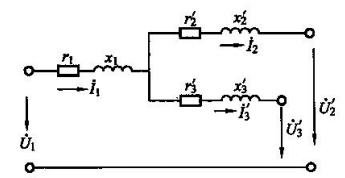
\includegraphics[width=0.80\textwidth]{5-9.png}
	\caption{三绕组变压器的等效电路}
	\label{fig_5-9}
\end{figure}

\subsection{参数的设定}

为了测定三个绕组的电阻和等效电抗,可做三个短路试验。
(1)电压加至绕组1,绕组2短路,绕组3开路,接线图与等效电路如图\ref{fig_5-10}(a)所示。测量${{U}_{k12}}{{I}_{k12}}$和${{p}_{k12}}$,可计算得
\begin{align}
& {{r}_{k12}}={{r}_{1}}+{{{{r}'}}_{2}} \\ 
& {{x}_{k12}}={{x}_{1}}+{{{{x}'}}_{2}} 
\label{5-39}
\end{align}
\begin{figure}[H]
	\centering
	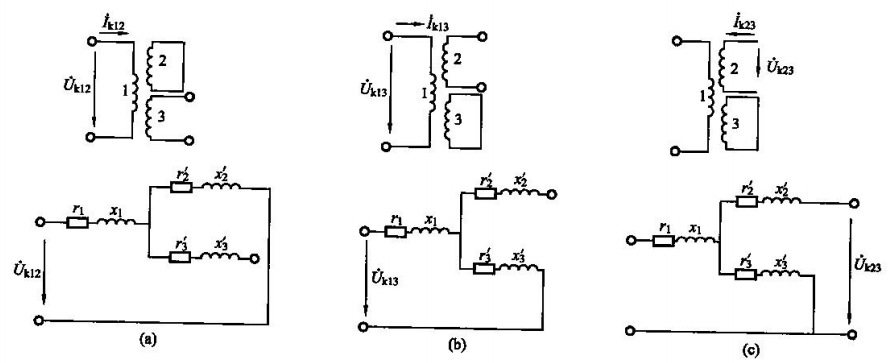
\includegraphics[width=0.80\textwidth]{5-10.png}
	\caption{三绕组变压器的短路试验}
	\label{fig_5-10}
\end{figure}

(2)加电压至绕组1,绕组3短路,绕组2开路[见图\ref{fig_5-10}(b)]。测量${{U}_{k13}}{{I}_{k13}}$和${{p}_{k13}}$,可计算得
\begin{align}
& {{r}_{k13}}={{r}_{1}}+{{{{r}'}}_{3}} \\ 
& {{x}_{k13}}={{{{x}'}}_{1}}+{{{{x}'}}_{3}} 
\label{5-40}
\end{align} 
(3)电压加至绕组2,绕组3短路,绕组1开路[见图\ref{fig_5-10}(c)]。测量${{U}_{k23}}{{I}_{k23}}$和${{p}_{k23}}$,可计算出${{r}_{k23}}$和${{x}_{k23}}$。但他们都是在绕组2上测得的值,为了归算到绕组1,还要乘以$k_{12}^{2}$,即有
\begin{align}
& k_{12}^{2}{{r}_{k23}}={{{{r}'}}_{2}}+{{{{r}'}}_{3}} \\ 
& k_{12}^{2}{{r}_{k23}}={{{{x}'}}_{2}}+{{{{x}'}}_{3}}
\label{5-41}
\end{align} 

将式(\ref{5-39})和式(\ref{5-40})中的电阻、电抗分别相加,再分别减去式(\ref{5-41})中的电阻、电抗,可得
\begin{align}
& {{r}_{1}}=\frac{{{r}_{k12}}+{{r}_{k13}}-k_{12}^{2}{{r}_{k23}}}{2} \\ 
& {{x}_{1}}=\frac{{{x}_{k12}}+{{x}_{k13}}-k_{12}^{2}{{x}_{k23}}}{2} 
\label{5-42}
\end{align}
同理可得
\begin{align}
& {{{{r}'}}_{2}}=\frac{{{r}_{k12}}+k_{12}^{2}{{r}_{k23}}-{{r}_{k13}}}{2} \\ 
& {{{{x}'}}_{2}}=\frac{{{x}_{k12}}+k_{12}^{2}{{x}_{k23}}-{{x}_{k13}}}{2} 
\label{5-43} 
\end{align}	
\begin{align}
& {{{{r}'}}_{3}}=\frac{{{r}_{k13}}+k_{12}^{2}{{r}_{k23}}-{{r}_{k12}}}{2} \\ 
& {{{{x}'}}_{3}}=\frac{{{x}_{k13}}+k_{12}^{2}{{x}_{k23}}-{{x}_{k12}}}{2}  
\label{5-44}
\end{align} 

\section{互感器}

互感器分电压互感器和电流互感器两种,它们的基本作用原理与变压器相同。使用互感 器有两个目的:一是使测量和保护电路与高压电网隔离,以保证工作人员和设备的安全;二是将高电压和大电流变换为低电压与小电流,以便于测量和为各种继电保护装置提供控制信 号。为了使用上的方便,电压互感器的二次侧额定电压都统一设计为100V;电流互感器的 二次侧额定电流都统一设计为5A或1A。
\subsubsection{电压互感器}

图\ref{fig_5-10}所示为电压互感器接线图。高压绕组并接于被测系统, 低压绕组接测量仪表或继电器的电压线圈。如需同时接数个线圈,则应将它们并联接在二次侧上。由于电压线圈的阻抗很大,所以电压互感器工作时接近于变压器的空载运行状态。

与普通变压器相比,电压互感器的主要作用不是传递功率,而是准确地改变电压。即要求二次侧电压${{\dot{U}}_{2}}$在大小和相位上能准确地代表一次侧电压${{\dot{U}}_{1}}$。变压器一、二次侧电压与匝数成正比的结论是在忽略一、二次侧漏阻抗的条件下得出的。而电压互感器工作时,${{\dot{I}}_{2}}\approx 0{{I}_{1}}\approx {{I}_{0}}$,为减少误差,在设计时应当注意以下两点。 

(1)尽量减小空载电流${{I}_{0}}$,为此铁心应采用导磁率高的硅钢片,并使磁路不饱和,磁通密度一般取0.6\textasciitilde0.8T。

(2)减小一、二次侧的漏阻抗,为此在绕组安排上应最大限度地减小它们间的漏磁通;另外绕组的导线也不能太细,以保证有较小的内阻。

\begin{figure}[H]
	\centering
	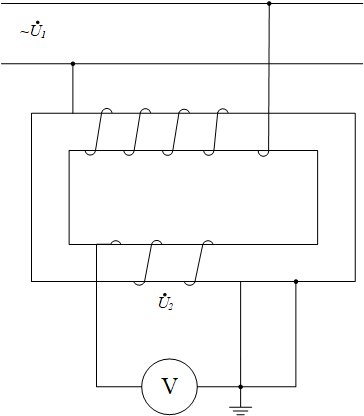
\includegraphics[width=0.80\textwidth]{5-11G.png}
	\caption{电压互感器接线图}
	\label{fig_5-11}
\end{figure}
\subsubsection{电流互感器}

图\ref{fig_5-11}所示为电流互感器接线图。一次侧串接于被测系统,二次侧接测量仪表或继电器的电流线圈。如需同时接数个线圈,则应将它们串联接在二次侧上。由于电流线圈的阻抗极小,所以电流互感器工作时,接近于变压器的短路状态。

为了将大电流变换为小电流,电流互感器二次侧的匝数较多,而一次侧的匝数较少,有时只有一匝。变压器一、二次侧电流与匝数成反比的结论是在忽略励磁电流的条件下得出的。为了使二次侧电流${{\dot{I}}_{2}}$能在大小和相位上更准确地反映一次侧电流${{\dot{I}}_{1}}$,必须尽量减小电流互感器的励磁电流。因此,在设计时应考虑以下两点。

(1)减小铁心中的磁通密度,使其比在电压互感器中更低,通常取0.08\textasciitilde0.1T。

(2)尽量减小绕组的漏抗和电阻,因为绕组的漏抗大,将使一次侧的端电压升高,进而引起磁通和励磁电流的增加。

电流互感器在使用时还应注意以下三点。

(1)二次侧所接电流线圈的数量不能超过规定的允许值。如串联线圈过多,将使二次侧端电压升高,并引起一次侧端电压升高,进而使磁通和励磁电流增大。

(2)在运行中绝对不允许二次侧开路。因为一次侧电流取决于被测电路中的电摞和负载,它不随二次侧电流的改变而变化。在正常运行时,由于二次侧电流的去磁作用,铁心中 的磁通很小;而当二次侧开路时,一次侧电流全部成为励磁电流,使铁心中磁通急剧增大,引起铁心严重过热。另外,在匝数较多的二次侧将感生很高的电压,这不仅可能造成绝缘的 损坏,同时还可能危及操作人员的安全。

(3) 为了操作人员和设备的安全,铁心和二次侧的一端应可靠地接地。

\begin{figure}[H]
	\centering
	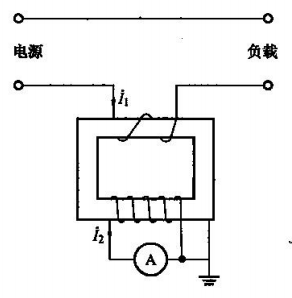
\includegraphics[width=0.80\textwidth]{5-12.png}
	\caption{电流互感器接线图}
	\label{fig_5-12}
\end{figure}

\end{document}